\documentclass[]{article}

%opening
\title{4F13 Probabilistic Machine Learning - True Skill Ranking}
\author{Lawrence Tray \\ St John's College}

%packages
\usepackage[margin=0.5in]{geometry}
\usepackage[export]{adjustbox}
\usepackage{graphicx}
\usepackage{amsmath}
\usepackage{amssymb}
\usepackage{hyperref}
\usepackage{caption}
\usepackage{subcaption}
\usepackage{parskip}
\usepackage{listings}
\usepackage{pdfpages}

%package setup
\graphicspath{{./img/}}
\DeclareMathOperator*{\argmax}{arg\,max}
\DeclareMathOperator*{\argmin}{arg\,min}

%custom commands
\newcommand{\dft}{\mathcal{F}}
\newcommand{\idft}{\mathcal{F}^{-1}}
\newcommand{\Xcal}{\mathcal{X}}
\newcommand{\Ncal}{\mathcal{N}}
\newcommand{\cmplx}{\mathbb{C}}
\newcommand{\Lcal}{\mathcal{L}}
\newcommand{\indep}{\perp \!\!\! \perp}
\newcommand{\figwidth}{0.6\linewidth}

%section numbering
\renewcommand{\thesubsection}{\thesection.\alph{subsection}}

\begin{document}

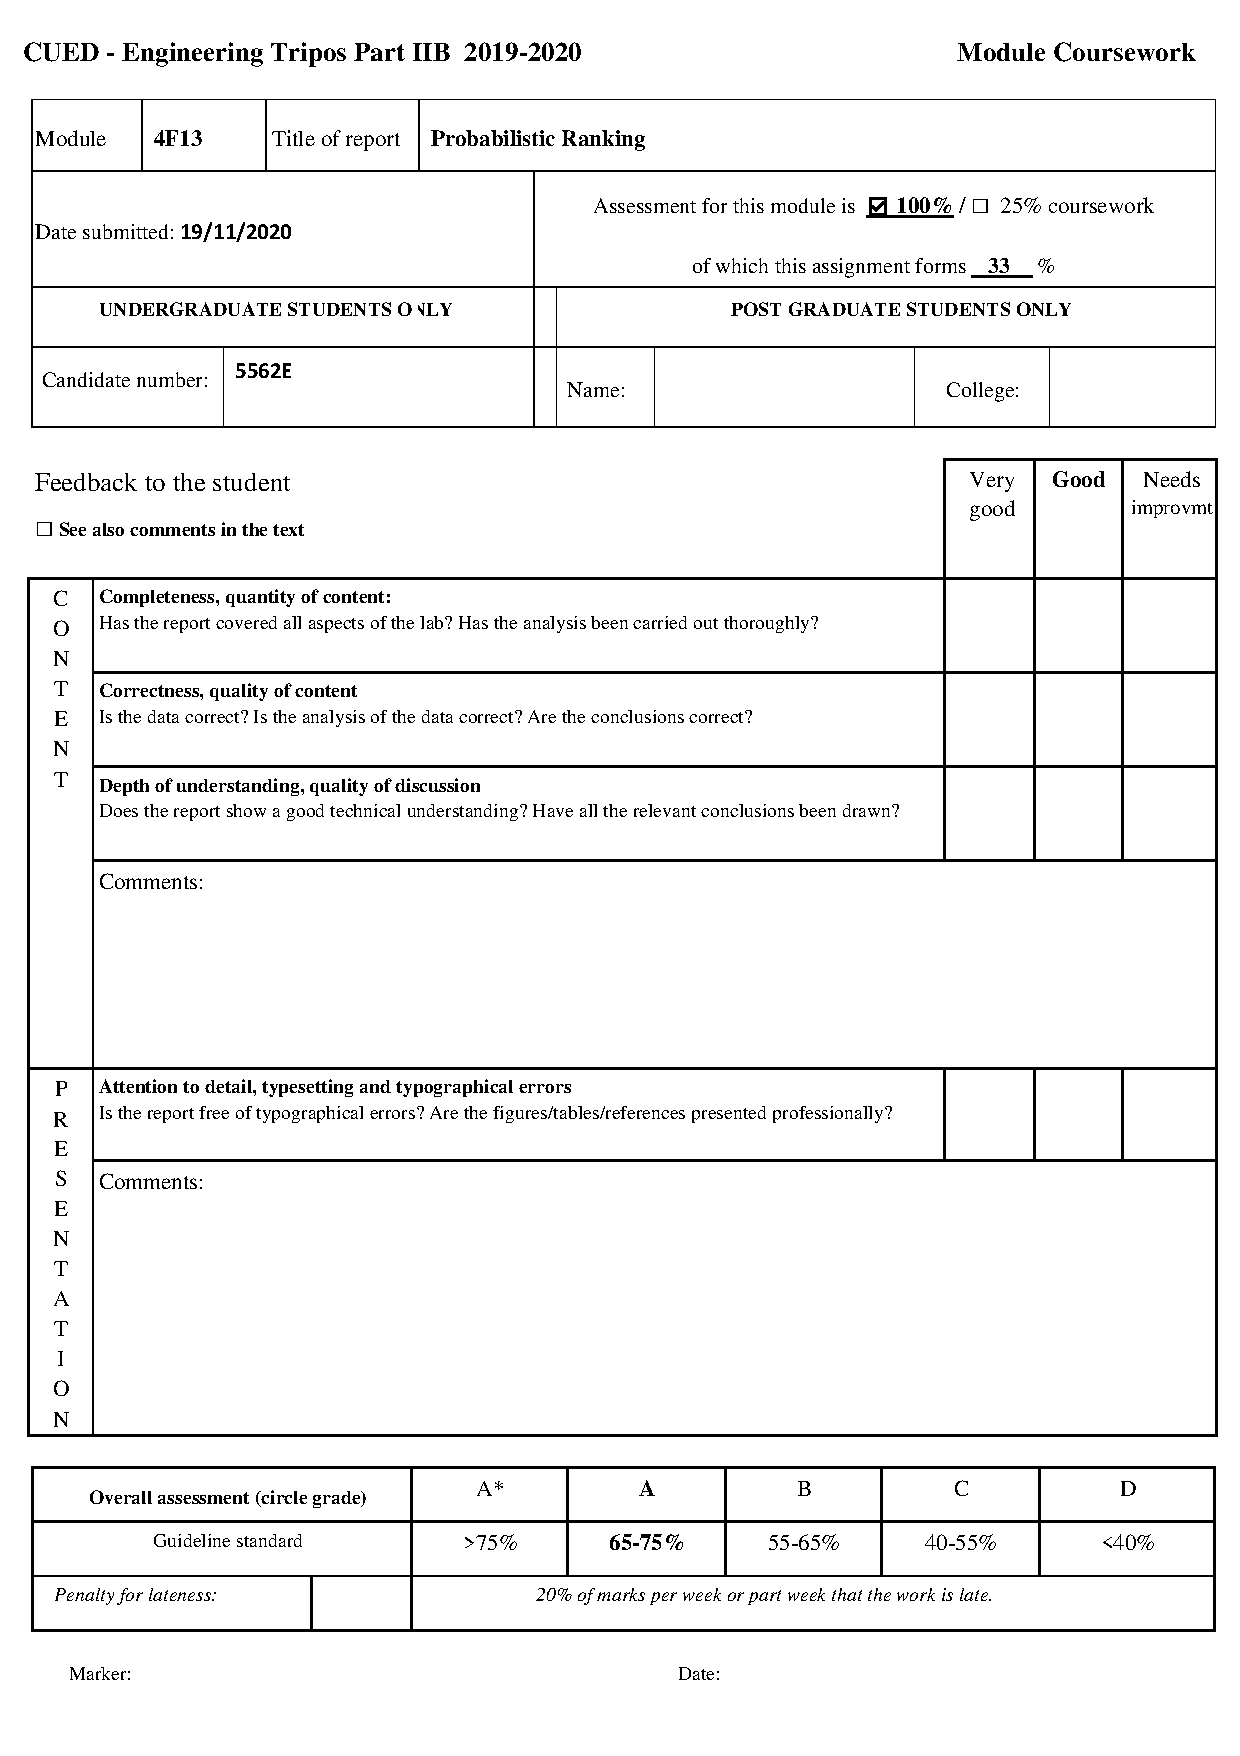
\includepdf[pages={1}]{coversheet-CW2.pdf}

\setcounter{page}{1}
\maketitle

\begin{abstract}
This report outlines the results of the second coursework for 4F13. 
\end{abstract}

\tableofcontents

\section{Questions}
\subsection{Gibbs Sampling}

Gibbs sampling is used to sample from a multi-variate distribution by sequentially sampling from univariate conditionals. In the True-Skill model, we can approximate the conditional distribution with a 1-D Gaussian of a certain mean and variance - which are functions of the other variables. The modified code to compute these samples is given in listing \ref{lst:gibbs}.

\begin{lstlisting}[frame=single, caption={Gibbs sampling additions}, label={lst:gibbs}, language={python}]
m = np.zeros((M, 1))
for p in range(M):
	# fill in m[p] prediction (natural param conditional)
	wins_array = np.array(G[:, 0] == p).astype(int)
	loss_array = np.array(G[:, 1] == p).astype(int)
	m[p] = np.dot(t[:,0], (wins_array - loss_array))
	
iS = np.zeros((M, M))  # Container for sum of precision matrices (likelihood terms)
for g in range(N):
	# Build the iS matrix
	winner = G[g, 0]
	loser = G[g, 1]
	
	iS[winner, winner] += 1
	iS[winner, loser] -= 1
	iS[loser, winner] -= 1
	iS[loser, loser] += 1
\end{lstlisting}

We plot the sampled player skills for a few players (figure \ref{fig:skill-samples-long}). These data do appear noisy (in some sense random) but it appears that neighbouring samples are strongly correlated. Furthermore it is hard to tell how soon the Gibbs sampler transitions into a stable probability density region.

\begin{figure}[!h]
	\centering
	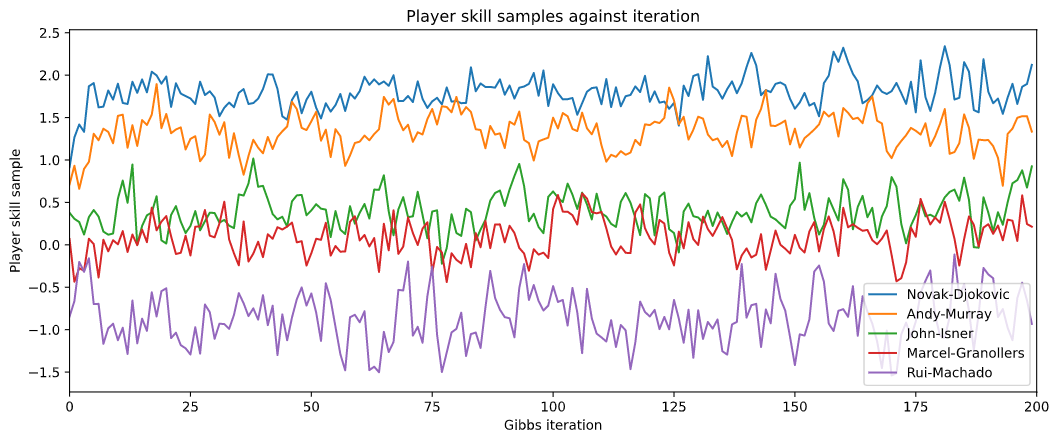
\includegraphics[width=\linewidth]{skill-samples-long.png}
	\caption{Gibbs skill samples for various players}
	\label{fig:skill-samples-long}
\end{figure}

To investigate the burn-in time (iterations until the Gibbs is in a stationary state), we can plot the population mean and standard deviation at each Gibbs iteration - figure \ref{fig:burn-in}. The population mean gives us little information but we see that the standard deviation converges to a steady value fairly quickly (only after 10 iterations). We can therefore set the burn-in time to $b=10$ and we would discard all preceding samples. 

\begin{figure}[!h]
	\centering
	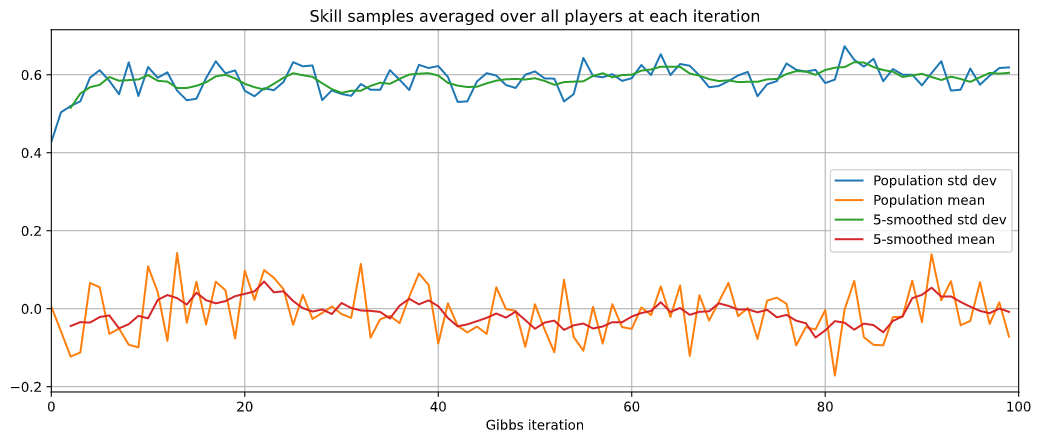
\includegraphics[width=\linewidth]{burn-in.png}
	\caption{Gibbs skill samples averaged over all players at each iteration}
	\label{fig:burn-in}
\end{figure}

However, there is an additional wrinkle, the plot in figure \ref{fig:skill-samples-long} is smoother than it should be; neighbouring samples are not independent. To test this hypothesis, we plot the auto-correlation of each player's skill samples (figure \ref{fig:auto-cor}). For samples to be approximately independent, their correlation should be close to 0. This is only true for all players for an offset of at least $k=10$. Nevertheless, we get good enough for $k=5$ - excepting one player: Djokovic.

\begin{figure}[!h]
	\centering
	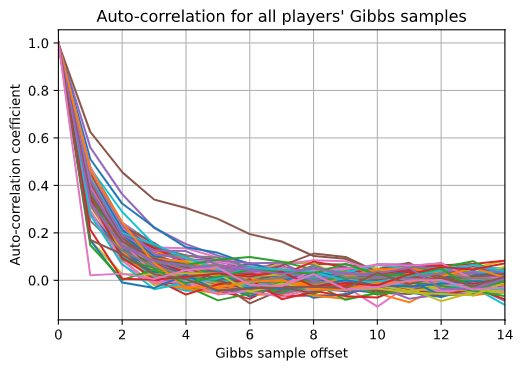
\includegraphics[width=\figwidth]{auto-cor.png}
	\caption{Auto-correlation for Gibbs sampler for all players}
	\label{fig:auto-cor}
\end{figure}

In summary, to run our Gibbs sampler efficiently and reliably, we only use samples after a burn-in period of $b=10$ iterations. Even then, we thin the samples such that we only keep every $t$'th ($t=5$) sample to ensure that they are approximately independent. We use these values $b=10$ and $t=5$ for the rest of the report - such that for 1100 samples we only keep 218 of them.

\subsection{EP - Message Passing}


\begin{figure}[!h]
	\begin{subfigure}{0.5\linewidth}
		\centering
		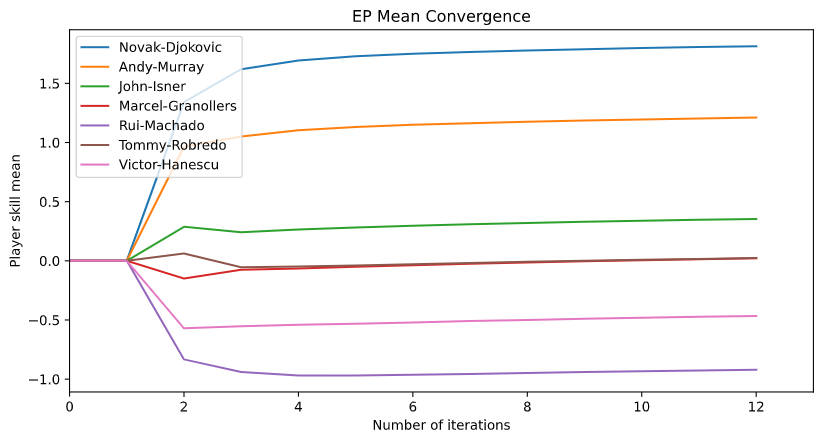
\includegraphics[width=\linewidth]{ep-mean.png}
		\caption{EP player skill mean evolution}
		\label{fig:ep-mean}
	\end{subfigure}
	\begin{subfigure}{0.5\linewidth}
		\centering
		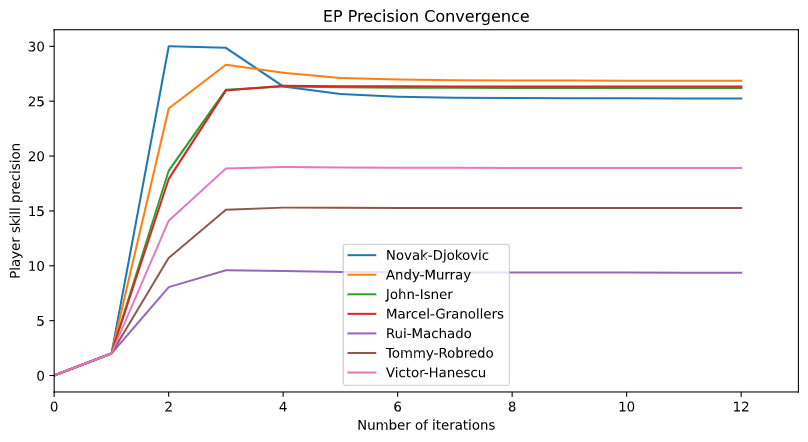
\includegraphics[width=\linewidth]{ep-precision.png}
		\caption{EP player skill precision evolution}
		\label{fig:ep-precision}
	\end{subfigure}
	\caption{EP player skill parameter evolution against iteration}
	\label{fig:ep-evolution}
\end{figure}


\subsection{EP - Top Four Head to Head}

Suppose that a player $i$ goes up against $j$. In the True-Skill model, we denote their skill by $w_i \sim \Ncal(m_i, \sigma_i^2)$ and $w_j \sim \Ncal(m_j, \sigma_j^2)$ respectively. The mean and variance parameters are estimated through message passing (the variance is just the inverse of the precision). 

The performance difference $s_{ij} = w_i - w_j$ is corrupted by Gaussian noise of unit variance $t_{ij} = s_{ij} + n$ to account for performance inconsistency ($n \sim \Ncal(0, 1)$). The match result is then given by the sign of $t_{ij}$ such that $t_{ij} > 0 \Rightarrow i \text{ wins}$ and j wins otherwise.

Having run message-passing, we wish to compute the probability that $i$ is more skilful than $j$: $P(s_{ij} > 0)$. This is different from the probability that $i$ beats $j$ in a head-to-head: $P(t_{ij} > 0)$. These probabilities are easy to compute by assuming that $w_i \indep w_j \indep n \indep w_i$, so means and variances combine additively:

\begin{align}
		s_{ij} = w_i - w_j &\sim \Ncal(m_i - m_j, \sigma_i^2 + \sigma_j^2)
		\label{eqn:s-ij} \\	
		t_{ij} = s_{ij} + n &\sim \Ncal(m_i - m_j, \sigma_i^2 + \sigma_j^2 + 1)
		\label{eqn:t-ij}
\end{align}

For any Gaussian r.v. $X \sim \Ncal(\mu, \sigma^2)$, $P(X > 0) = \Phi(\mu / \sigma)$ - where $\Phi(\cdot)$ is the standard Gaussian c.d.f. Applying this result to equations \ref{eqn:s-ij} and \ref{eqn:t-ij} for the top four ranked players, we obtain table \ref{tab:top-4}.

\begin{table}[!h]
	\subfloat[Prob. row player is more skilful]{
		\begin{tabular}{c | c c c c}
			$P(s_{ij} > 0)$ & \textbf{Djokovic} & \textbf{Federer} & \textbf{Nadal} & \textbf{Murray} \\ \hline
			\textbf{Djokovic}      & -                 & 0.91             & 0.94           & 0.99            \\
			\textbf{Federer}       & 0.09              & -                & 0.58           & 0.81            \\
			\textbf{Nadal}         & 0.06              & 0.42             & -              & 0.76            \\
			\textbf{Murray}        & 0.01              & 0.19             & 0.24           & -              
		\end{tabular}
	}
	\subfloat[Prob. row player wins a head-to-head]{
		\begin{tabular}{c | c c c c}
			$P(t_{ij} > 0)$ & \textbf{Djokovic} & \textbf{Federer} & \textbf{Nadal} & \textbf{Murray} \\ \hline
			\textbf{Djokovic}      & -                 & 0.64             & 0.66           & 0.72            \\
			\textbf{Federer}       & 0.36              & -                & 0.52           & 0.59            \\
			\textbf{Nadal}         & 0.34              & 0.48             & -              & 0.57            \\
			\textbf{Murray}        & 0.28              & 0.41             & 0.43           & -              
		\end{tabular}
	}
	\caption{Top four players comparison based on EP (5 iterations)}
	\label{tab:top-4}
\end{table}

We clearly see that the probability of player $i$ being more skilful than $j$ is always more extreme (further from 0.5) than the probability of winning a head-to-head. This makes sense mathematically as the variance $V[t_{ij}] > V[s_{ij}]$. It also makes sense intuitively because an individual match is subject to performance variation. If I were to play a single point against Federer, I might win. However, as the number of points increases the chance of winning the majority falls to (in my case) 0. This is the difference between being a better player and just getting lucky.

If Djokovic played an infinite number of matches against Murray, a priori we can be 99\% confident that he will win the majority. However, we would expect Djokovic to only win 72\% of these matches - not 99\%.

\subsection{Gibbs - Nadal v Djokovic}

\begin{figure}[!h]
	\centering
	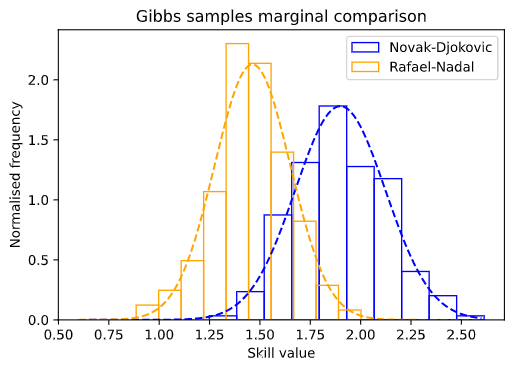
\includegraphics[width=\figwidth]{djokovic-nadal-marginal.png}
	\caption{Gibbs samples marginal comparison - Djokovic v Nadal}
	\label{fig:djok-nadal-marginal}
\end{figure}

\begin{figure}[!h]
	\centering
	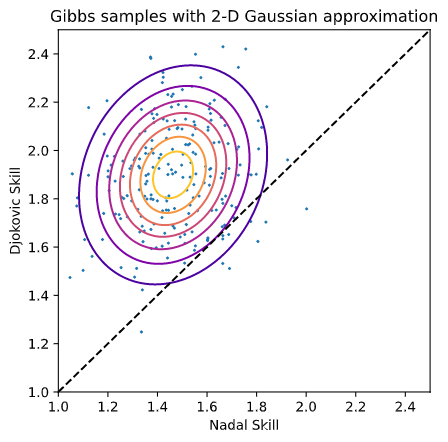
\includegraphics[width=\figwidth]{djokovic-nadal-joint.png}
	\caption{Gibbs samples joint comparison - Djokovic v Nadal}
	\label{fig:djok-nadal-joint}
\end{figure}

\begin{figure}[!h]
	\centering
	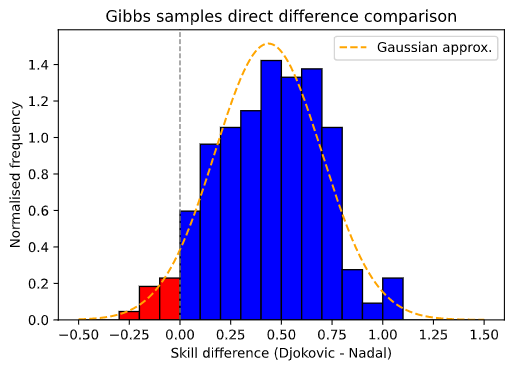
\includegraphics[width=\figwidth]{djokovic-nadal-diff.png}
	\caption{Gibbs samples direct difference comparison - Djokovic v Nadal}
	\label{fig:djok-nadal-diff}
\end{figure}



\subsection{Method Comparison: Win ratio, Gibbs and EP}

We go about ranking players using different methods: basic win ratio model; Gibbs sampling for True-Skill model; and EP estimates for True-Skill.

The win ratio model assumes that each player has a fixed probability of winning their match irrespective of their opponent. If a player has played $n$ and won $k$ of them we classify their win percentage $p \sim \Ncal(k/n, k(n-k)/n^2)$ - this applies standard results for combining $n$ independent Bernoulli r.v.'s. We plot the mean and standard deviation of $p$ on figure \ref{fig:win-ratio-ranking}.

With Gibbs sampling, we sample the player skill from conditional distributions and update the sample for each player at every iteration. We can restrict the samples to those produced after the burn-in period $b=20$ and thin further such that every $t$'th sample is kept $t=5$. This gives us a set of independent samples for the skill of each player and we can calculate the mean and variance of this set empirically (plotted on figure \ref{fig:gibbs-ranking}).

For Expectation Propagation, we run the Message Passing algorithm for 3 iterations as that is enough to achieve convergence. This algorithm returns the expected means and precisions (inverse variance) for the skill of each player and so we can plot these directly (figure \ref{fig:ep-ranking})

\begin{figure}[!h]
	\centering
	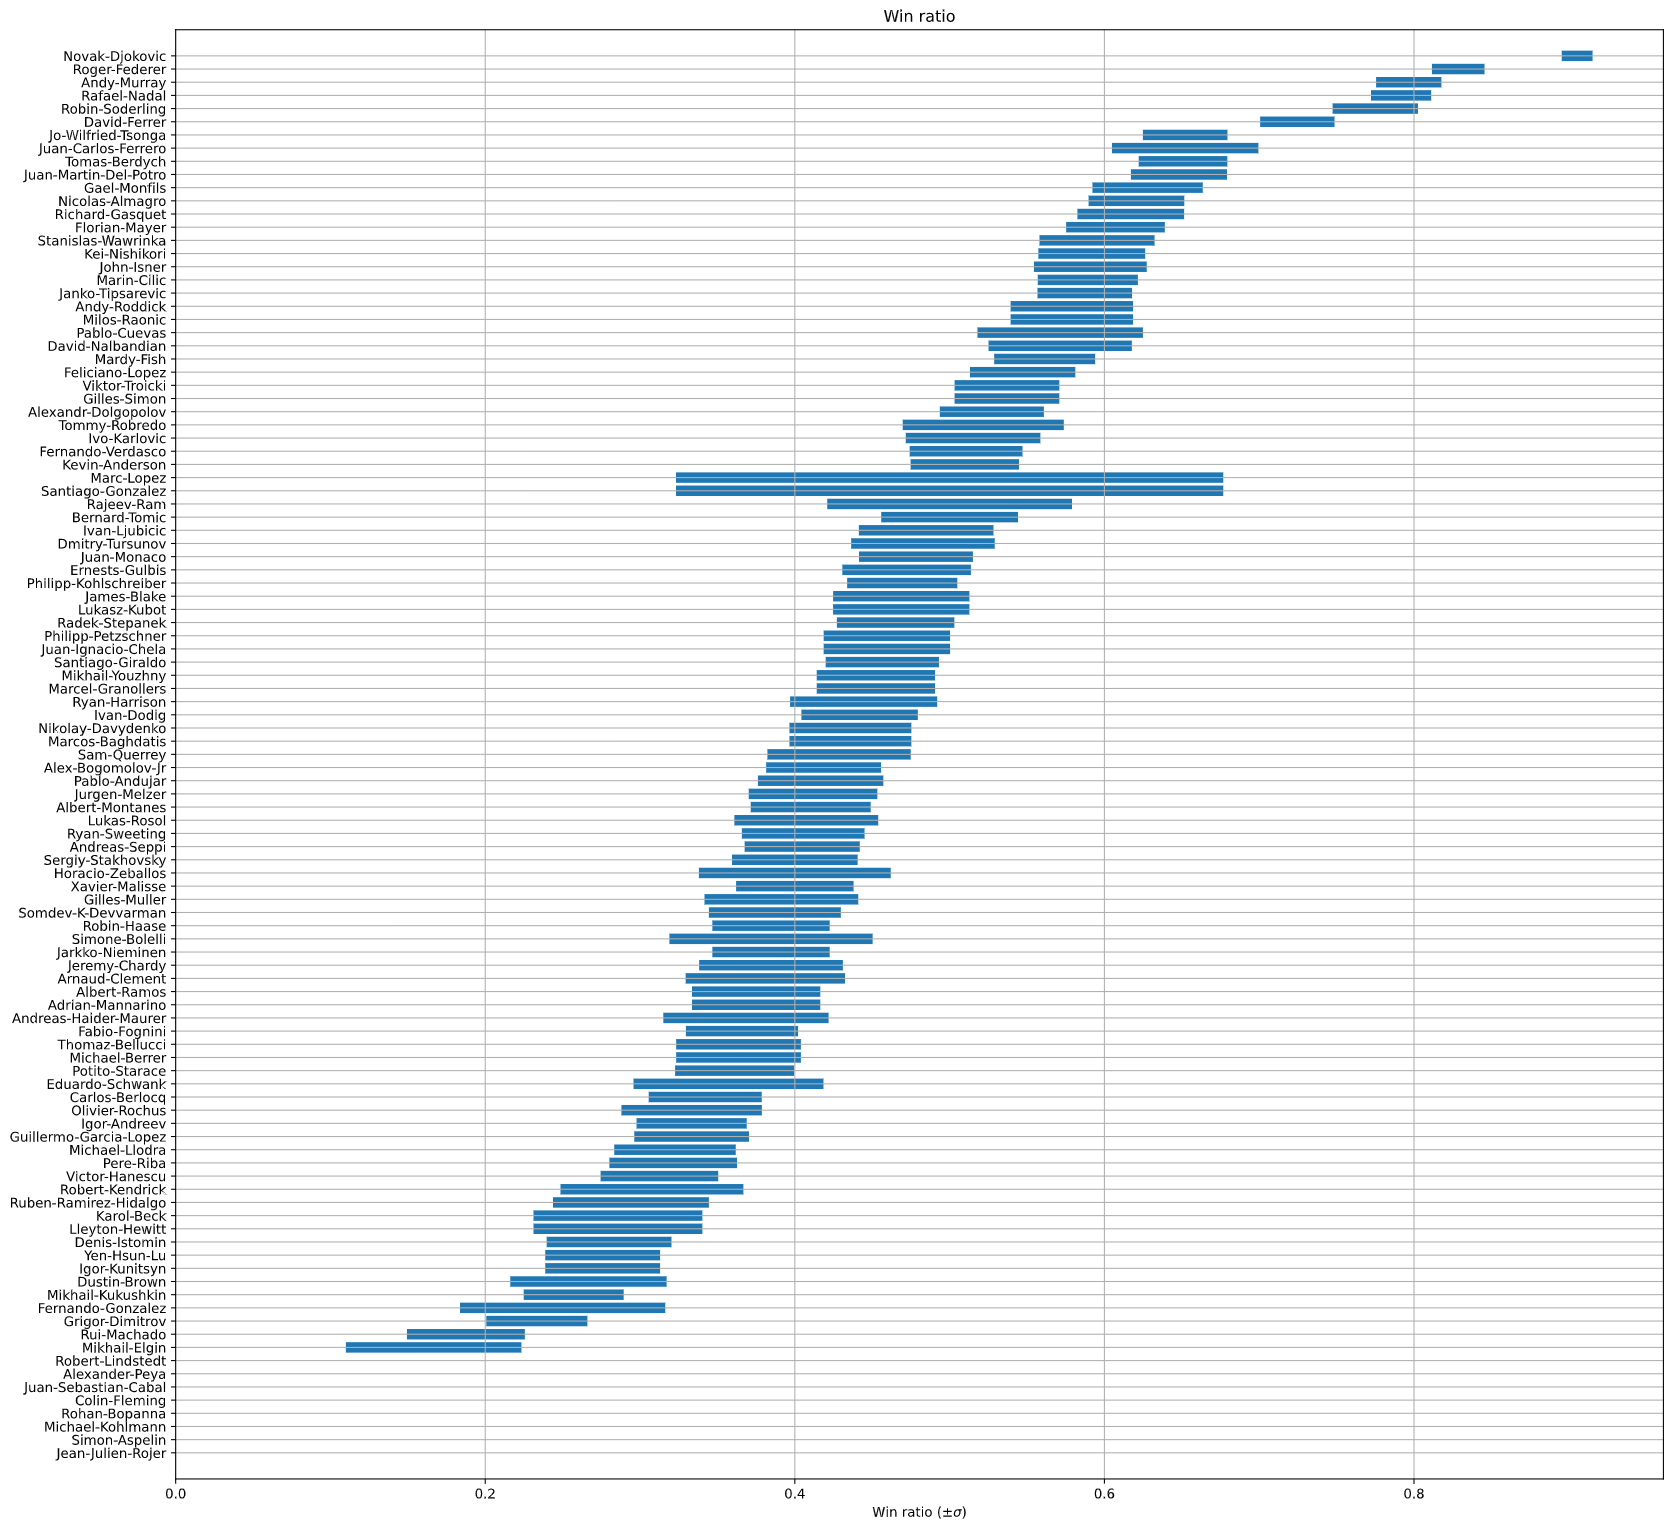
\includegraphics[width=\linewidth]{win-ratio.png}
	\caption{Player rankings by win ratio}
	\label{fig:win-ratio-ranking}
\end{figure}

\begin{figure}[!h]
	\centering
	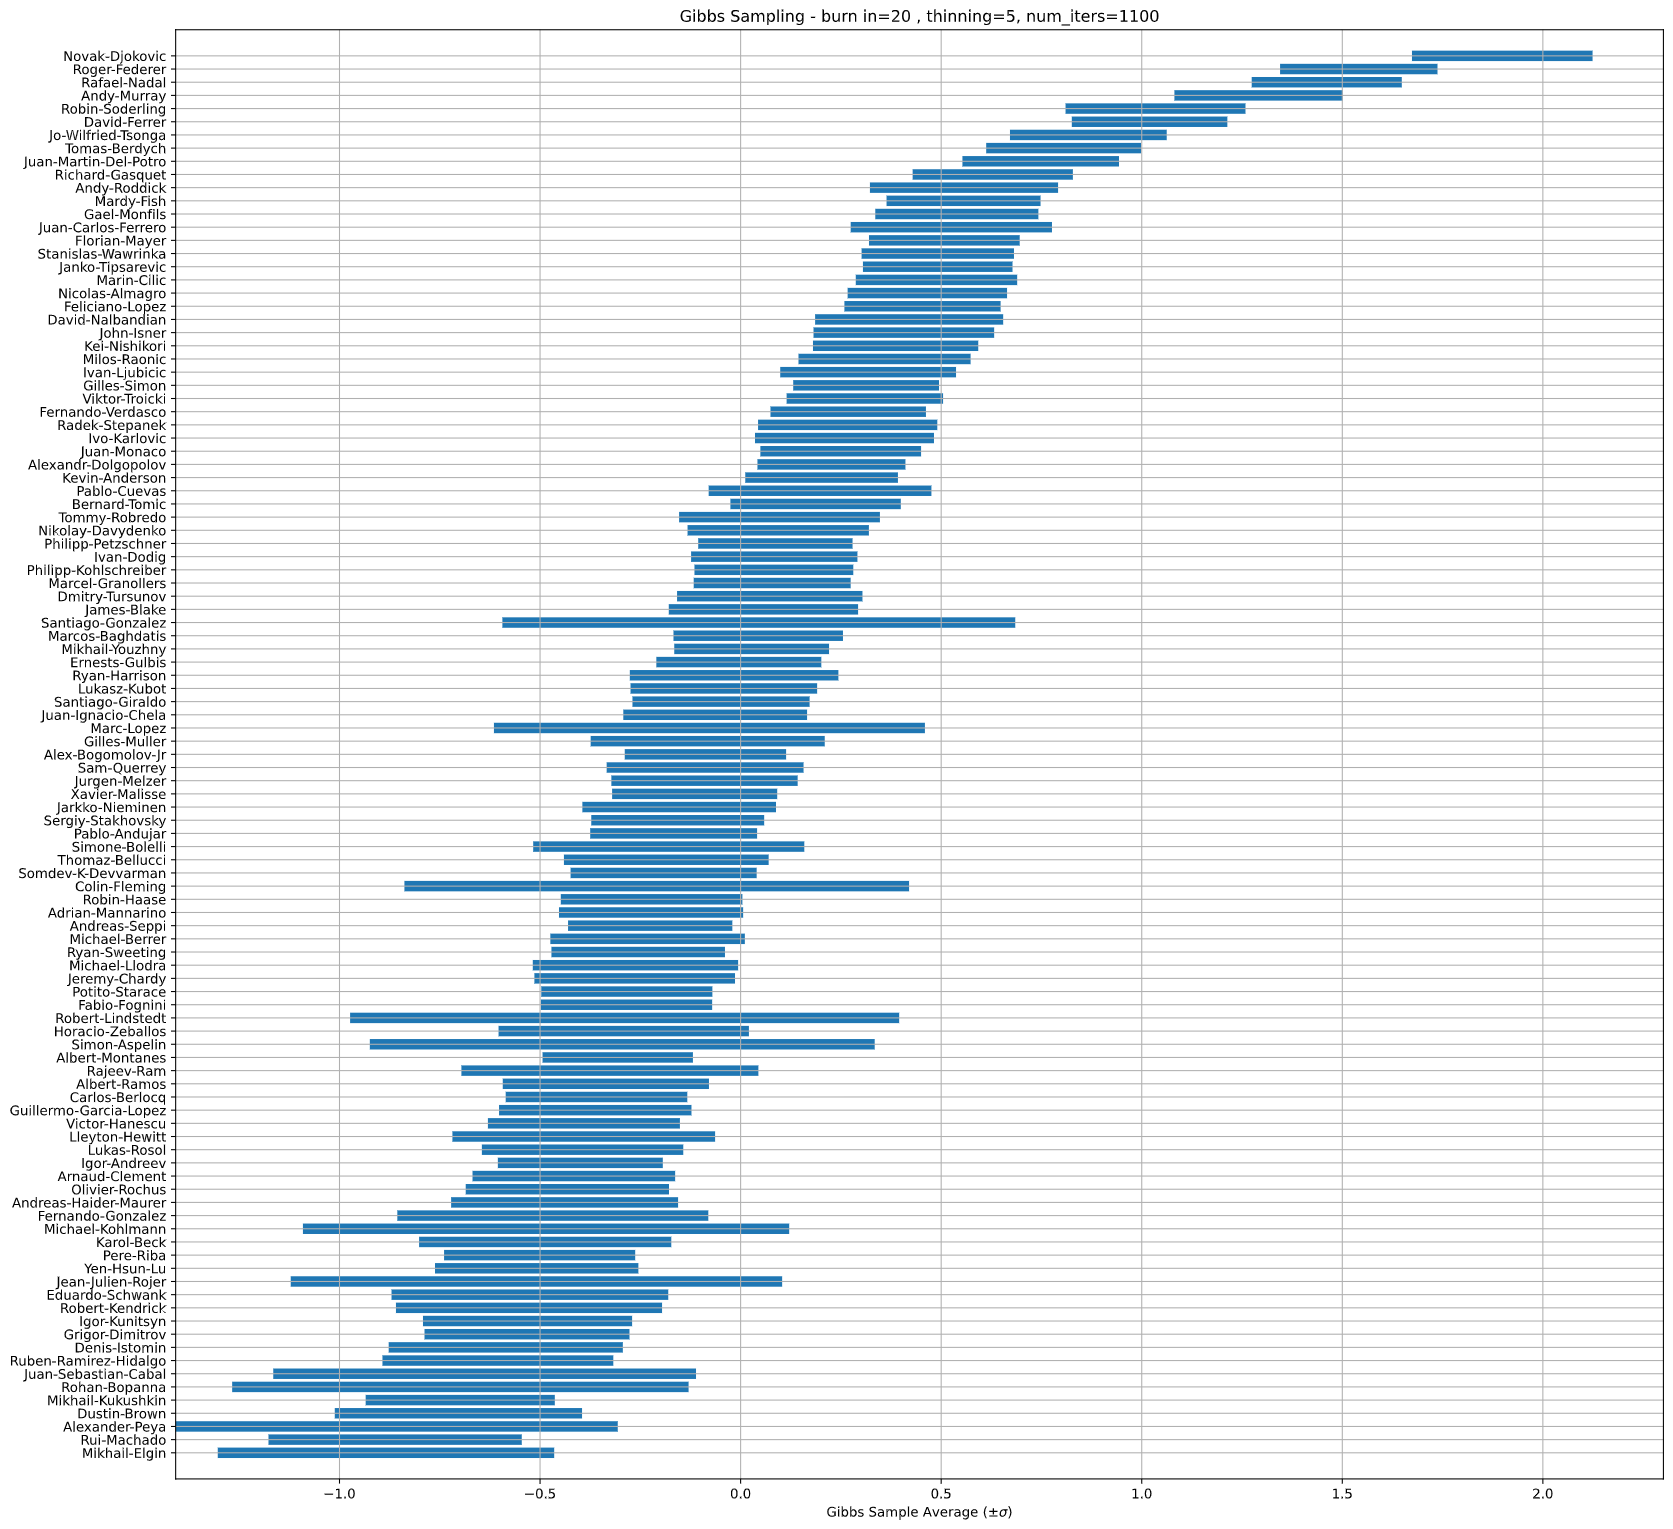
\includegraphics[width=\linewidth]{gibbs-ranking.png}
	\caption{Players rankings by mean of Gibbs skill samples}
	\label{fig:gibbs-ranking}
\end{figure}

\begin{figure}[!h]
	\centering
	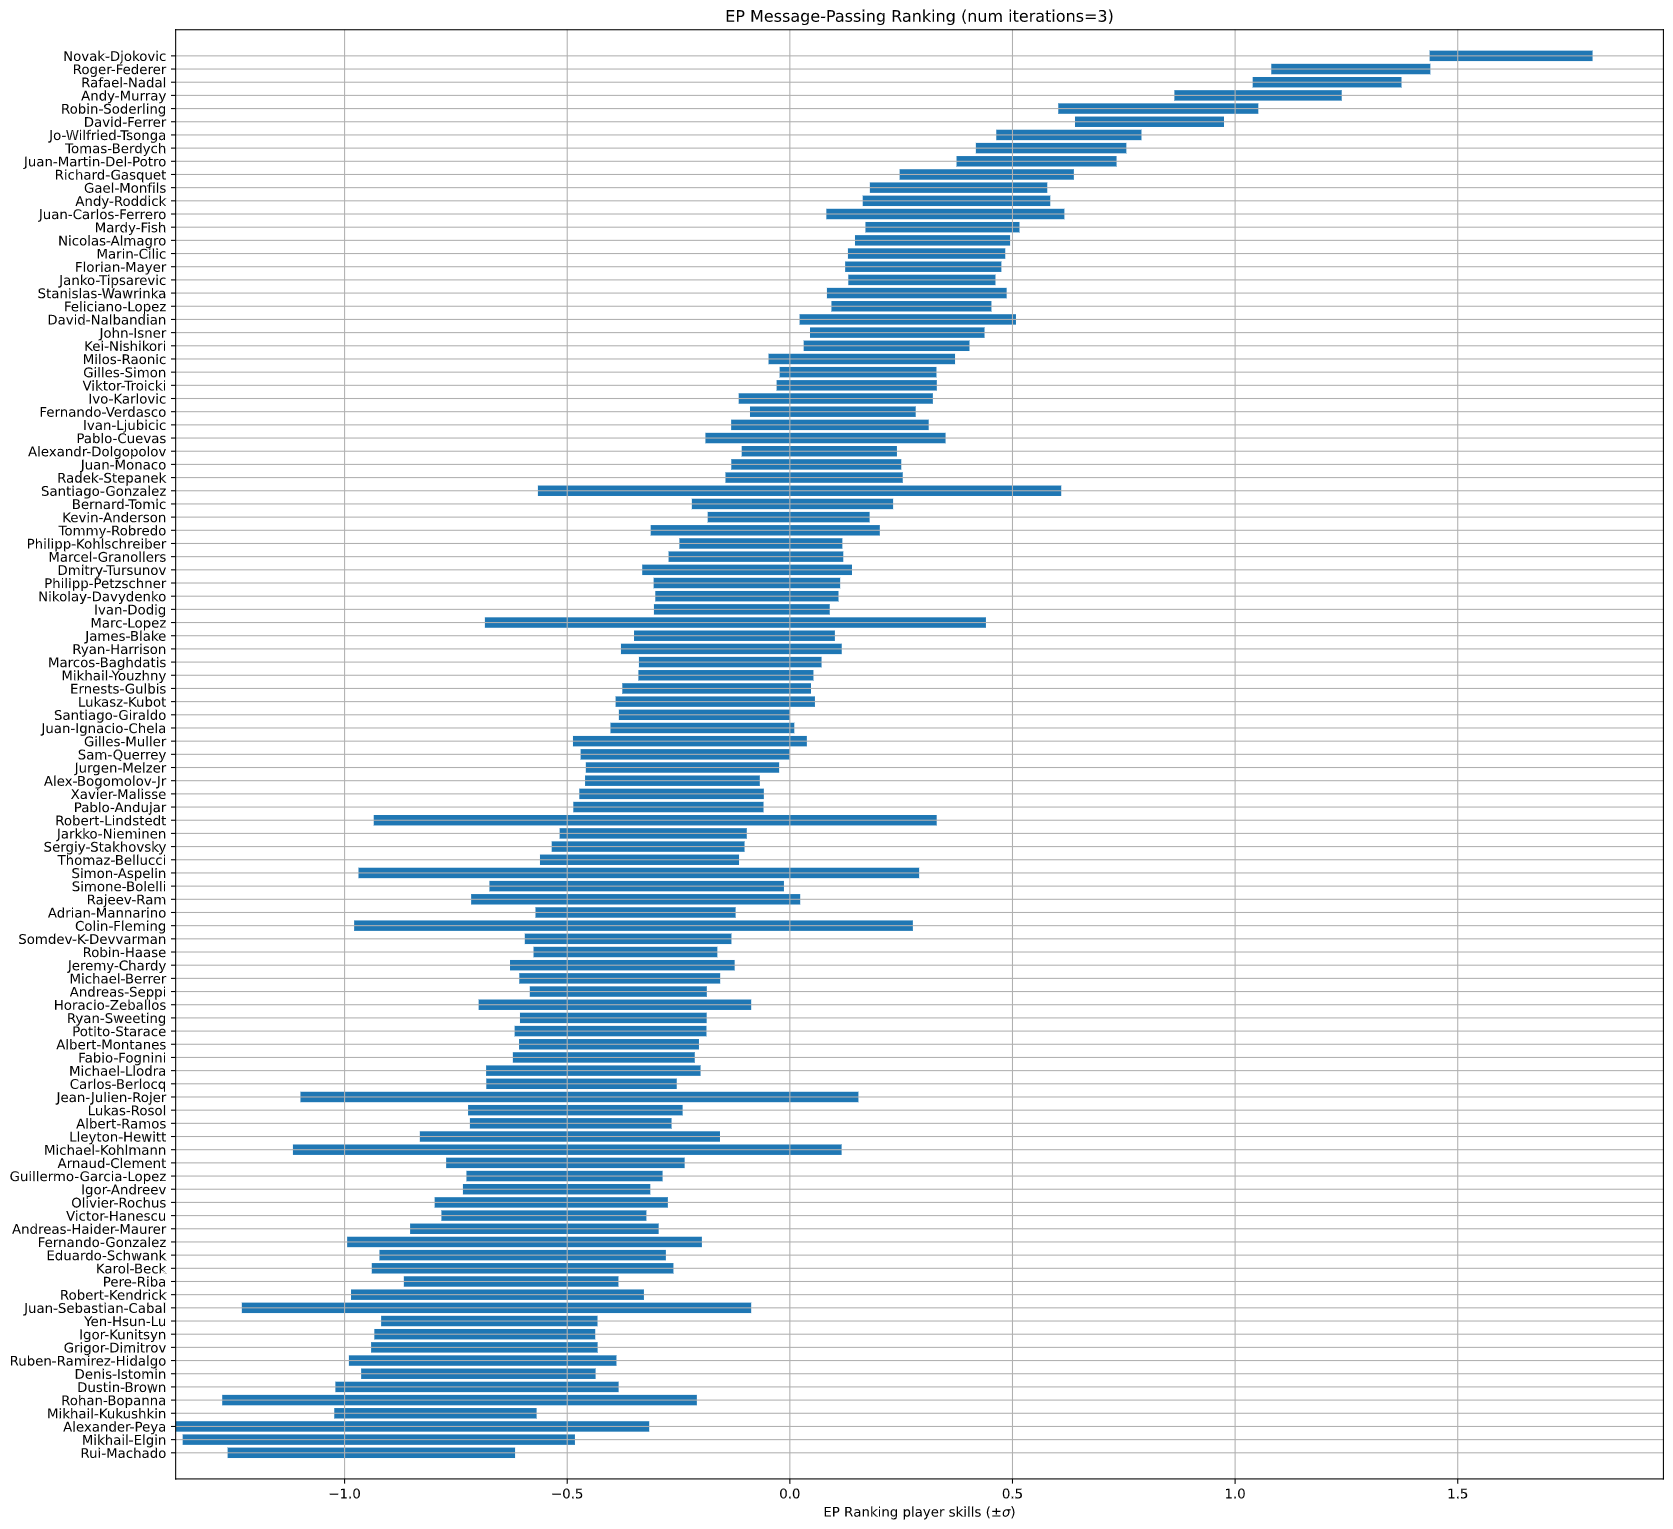
\includegraphics[width=\linewidth]{ep-ranking.png}
	\caption{Player rankings by mean of EP-estimated skills}
	\label{fig:ep-ranking}
\end{figure}

\textbf{Words}: XX

\end{document}
